\documentclass[12pt,a4paper,twoside,openright,titlepage,final]{article}
\usepackage{fontspec}
\usepackage{amsmath}
\usepackage{amsfonts}
\usepackage{amssymb}
\usepackage{makeidx}
\usepackage{graphicx}
\usepackage[hidelinks,unicode=true]{hyperref}
\usepackage[spanish,es-nodecimaldot,es-lcroman,es-tabla,es-noshorthands]{babel}
\usepackage[left=3cm,right=2cm, bottom=4cm]{geometry}
\usepackage{natbib}
\usepackage{microtype}
\usepackage{ifdraft}
\usepackage{verbatim}
\usepackage[nottoc]{tocbibind}
\usepackage{pdflscape}
\usepackage{fancyvrb}
\usepackage[obeyDraft]{todonotes}
\ifdraft{
	\usepackage{draftwatermark}
	\SetWatermarkText{BORRADOR}
	\SetWatermarkScale{0.7}
	\SetWatermarkColor{red}
}{}
\usepackage{booktabs}
\usepackage{longtable}
\usepackage{calc}
\usepackage{array}
\usepackage{caption}
\usepackage{subfigure}
\usepackage{footnote}
\usepackage{url}
\usepackage[titletoc]{appendix}

\setsansfont[Ligatures=TeX]{texgyreadventor}
\setmainfont[Ligatures=TeX]{texgyrepagella}
\setmonofont{FreeMono}

\usetikzlibrary{decorations.pathreplacing}

%*******************************************************
%                 NO MODIFICAR
\newcommand*{\FSfont}[1]{%
  \fontencoding{T1}\fontfamily{#1}\selectfont}

\newlength{\tpheight}\setlength{\tpheight}{0.9\textheight}
\newlength{\txtheight}\setlength{\txtheight}{0.9\tpheight}
\newlength{\tpwidth}\setlength{\tpwidth}{0.9\textwidth}
\newlength{\txtwidth}\setlength{\txtwidth}{0.9\tpwidth}
\newlength{\drop}
%*******************************************************

% Crea una portada con los siguientes parámetros
%
% #1 : Título 
% #2 : Subtítulo
% #3 : Subsubtítulo
% #4 : Autor(es)
% #5 : Lugar
%

\newcommand*{\portada}[5]{
\begin{titlepage}
\begingroup
\vspace*{1cm}
\drop = 0.2\txtheight
\centering
\vfill
{\Huge \scshape #1}\\[\baselineskip]
{\Large \textbf{#2}}\\[\baselineskip]
{\Large \scshape #3}\\[\baselineskip]
\vspace*{0.3cm}
{\large \textit{#4}}\\[0.5\drop]

\includegraphics[scale=0.35]{./imagenes/logoURJC.jpg}
\vspace*{1.5cm}

{\large \scshape #5, \today} \par
\begin{center}
\end{center}
\vfill\null
\endgroup
\end{titlepage}
}
 %*****************************************************
 


\author{José Ignacio Escribano}

\title{}

\setlength{\parindent}{0pt}

\begin{document}

\pagenumbering{alph}
\setcounter{page}{1}

\portada{Caso Práctico I}{Minería de datos}{Análisis de clústers}{José Ignacio Escribano}{Móstoles}

\listoffigures
\thispagestyle{empty}
\newpage

\listoftables
\thispagestyle{empty}
\newpage

\tableofcontents
\thispagestyle{empty}
\newpage


\pagenumbering{arabic}
\setcounter{page}{1}

\section{Introducción}

En este caso práctico aplicaremos la teoría vista para obtener grupos de países a partir de datos socioeconómicos usando el algoritmo de las k-medias. Por último, usaremos dendogramas para identificar tres tipos de iris a partir de la anchura y longitud de los pétalos y sépalos de sus hojas.

\section{Resolución de las cuestiones de evaluación}

A continuación resolveremos las cuestiones de evaluación planteadas.

\subsection{Cuestión 1}

En esta cuestión, utilizaremos los datos del fichero ``SocioeconomicDatasets.csv'', que contiene 6 variables que describen a 91 países. Estas variables son Birth.Rate (tasa de natalidad), Mortality.Rate (tasa de mortalidad), Infant.mortality.Rate (tasa de mortalidad infantil), Life.expectency.man (esperanza de vida en los hombres), Life.expectency.woman (esperanza de vida en mujeres) y GNP (Producto Interior Bruto).\\

Como en el caso resuelto, transformamos la variable GNP aplicando logaritmos. Renombramos la variable como logGNP. Además escalamos los datos, ya que cada variable tiene escalas distintas y afectará negativamente a la hora de calcular la matriz de distancias.\\

Aplicamos el algoritmos de las k-medias con $k=5$, es decir, agruparemos los países en 5 grupos, de acuerdo a las variables explicativas.\\

Los 5 centroides son los siguientes:

\begin{Verbatim}[fontsize=\footnotesize]
                             [,1]      [,2]        [,3]       [,4]       [,5]
Group.1                1.00000000  2.000000  3.00000000  4.0000000  5.0000000
Birth.Rate             0.43148667  1.273042 -0.69750278 -1.0993725  1.0732598
Mortality.Rate        -0.52272683  2.194461 -0.50506881 -0.4983267  0.7883010
Infant.mortality.Rate  0.25309057  1.925793 -0.72708079 -1.0011662  0.9011199
Life.expectency.man   -0.05682204 -2.024511  0.57326819  1.0367668 -0.9676394
Life.expectency.woman -0.13881053 -1.925379  0.64835233  1.0498822 -1.0104112
logGNP                -0.24674302 -1.387819 -0.04384888  1.3387075 -0.7900894
\end{Verbatim}


Representamos los clusters, representando las variables dos a dos, como se puede ver en la Figura~\ref{fig:pairs_plot}.\\

\begin{figure}[tbph!]
\centering
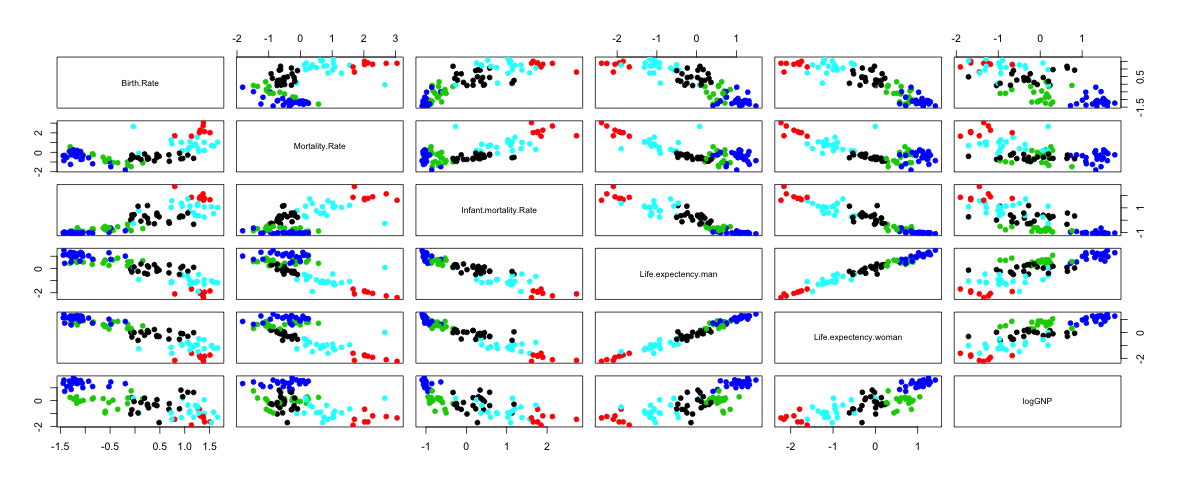
\includegraphics[width=0.8\linewidth]{imagenes/pairs_plot}
\caption{Clusters mediante la representación de las variables dos a dos}
\label{fig:pairs_plot}
\end{figure}

Este gráfico tiene difícil interpretabilidad, por lo que procedemos reduciendo la dimensión de los datos, haciendo uso del análisis de componentes principales. Así, los cinco clústers se pueden ver en la Figura~\ref{fig:plot_5clusters}.\\

\begin{figure}[tbph!]
\centering
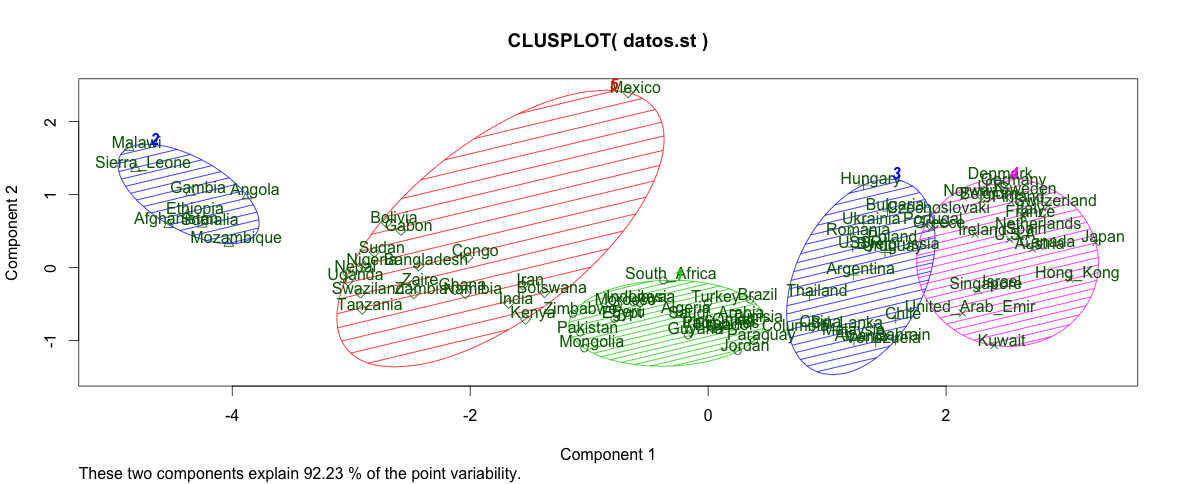
\includegraphics[width=0.8\linewidth]{imagenes/plot_5clusters}
\caption{Clusters mediante el análisis de componentes principales}
\label{fig:plot_5clusters}
\end{figure}

Este gráfico es mucho más explicativo que el anterior. Los países por grupos son los siguientes:

\begin{verbatim}
#-------------------------------------------------------------
# Grupo 1
#-------------------------------------------------------------
Brazil      Ecuador       Guyana     Paraguay      Peru         
Oman        Saudi_Arabia  Turkey     Indonesia     Mongolia     
Algeria     Egypt         Libya      Morocco       South_Africa 
Iraq        Jordan        Pakistan   Philippines   Tunisia    
Zimbabwe 

#-------------------------------------------------------------
# Grupo 2
#-------------------------------------------------------------
Afghanistan  Angola  Ethiopia   Gambia  Malawi   Mozambique 
Sierra_Leone Somalia 

#-------------------------------------------------------------
# Grupo 3
#-------------------------------------------------------------
Albania    Bulgaria  Czechoslovaki  Hungary      Poland       
Romania    USSR      Byelorussia    Ukrainia     Argentina         
Chile      Columbia  Uruguay        Venezuela    Bahrain         
China      Malaysia  Sri_Lanka      Thailand 

#-------------------------------------------------------------
# Grupo 4
#-------------------------------------------------------------
Belgium    Finland   Denmark        France        Germany           
Ireland    Italy     Netherlands    Norway        Portugal            
Greece     Spain     Sweden         Switzerland   U.K.          
Austria    Japan     Canada         U.S.A.        Israel           
Kuwait     Hong_Kong Singapore      United_Arab_Emir 

#-------------------------------------------------------------
# Grupo 5
#-------------------------------------------------------------
Bolivia     Mexico     Iran      Bangladesh India    Nepal   
Botswana    Congo      Gabon     Ghana      Kenya    Namibia    
Nigeria     Sudan      Swaziland Uganda     Tanzania  Zaire 
Zambia 
\end{verbatim}

\subsection{Cuestión 2}

En esta cuestión usaremos la base de datos \texttt{iris}, disponible en el paquete datasets de R. La base de datos describe tres tipos de iris (setosa, virginica y versicolor) a partir de las longitud y anchura de los pétalos y de los sépalos.\\

De esta base de datos, elegimos 50 para obtener 3 clusters. En este caso, usamos clusters jerárquicos.\\

Usamos la distancia euclídea para obtener la matriz de distancias.\\

Tenemos varios métodos de agrupación disponibles en R para obtener el dendograma. Usaremos todos para ver con cuál se obtiene una mejor clasificación.\\

Comenzamos con el método ward.D. El el dendograma obtenido con este método se puede ver en la Figura~\ref{fig:dendograma_ward.D}\\

\begin{figure}[tbph!]
\centering
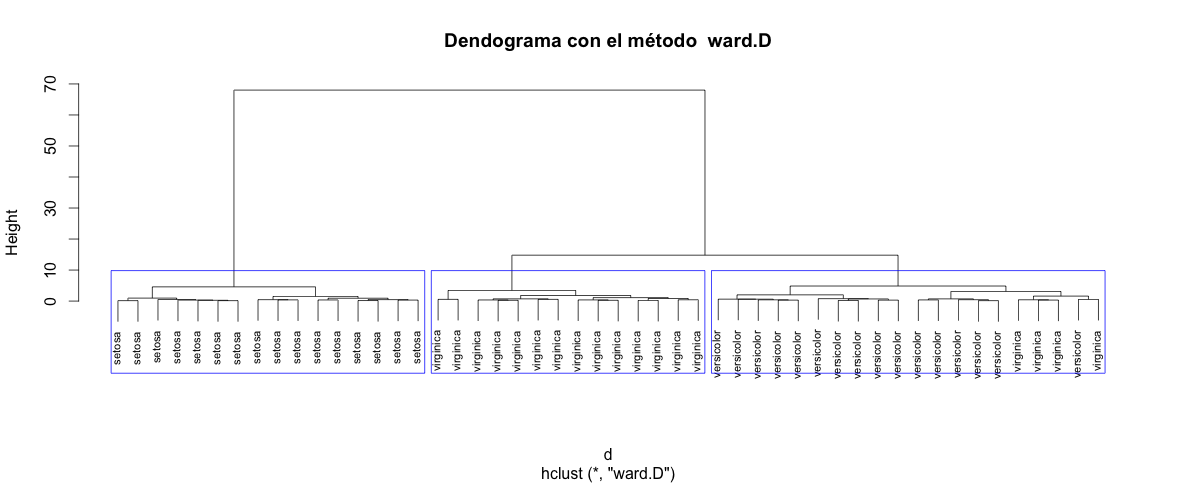
\includegraphics[width=0.9\linewidth]{imagenes/dendograma_wardD}
\caption{Dendograma con el método ward.D}
\label{fig:dendograma_ward.D}
\end{figure}

Con este método se detecta perfectamente la especie setosa, pero no se distingue la especie versicolor de la virginica.\\

Usamos ahora el método ward.D2, cuyo dendograma se muestra en la Figura~\ref{fig:dendograma_ward.D2}.\\

\begin{figure}[tbph!]
\centering
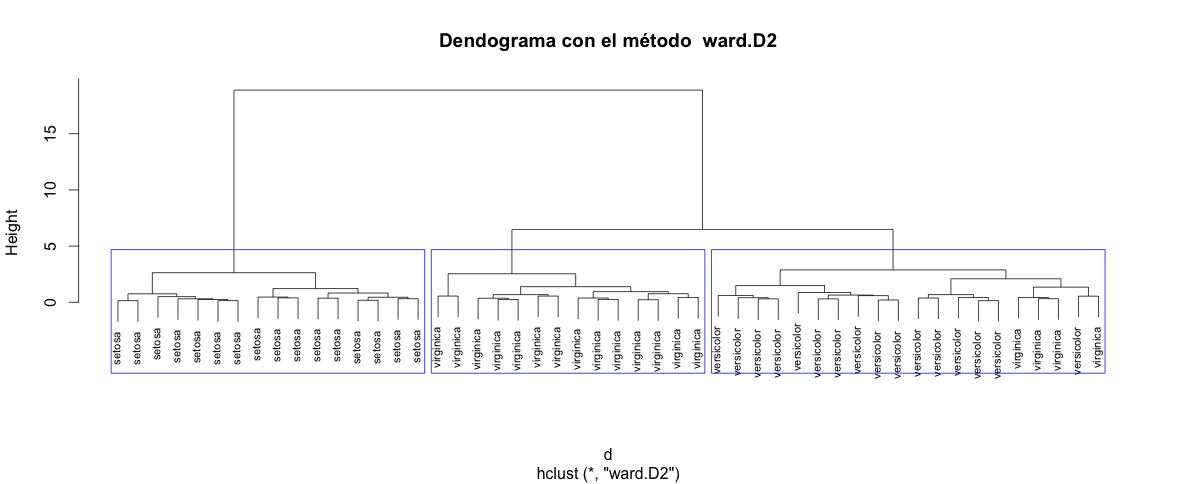
\includegraphics[width=0.9\linewidth]{imagenes/dendograma_wardD2}
\caption{Dendograma con el método ward.D2}
\label{fig:dendograma_ward.D2}
\end{figure}

De nuevo, se obtiene que se detecta perfectamente la especie setosa, pero se mezclan las especies versicolor y virginica en el tercer cluster, el que está a la derecha.\\

Si repetimos lo anterior con los métodos restantes (single, complete, average, mcquitty, median y centroid), obtenemos los mismos resultados: se detecta a la perfección la especie setosa, pero en un cluster se mezclan las especies virginica y versicolor. Ver Figura~\ref{fig:dendogramas_otros_metodos}.\\

\begin{figure}[htbp]
\centering
\subfigure[Método single]{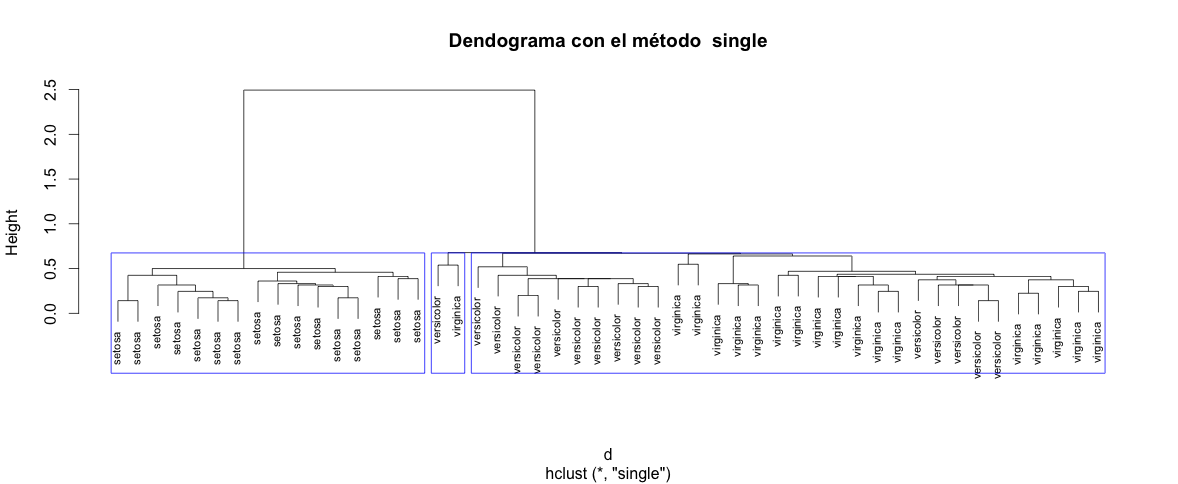
\includegraphics[width=0.45\linewidth]{imagenes/dendograma_single}}
\subfigure[Método complete]{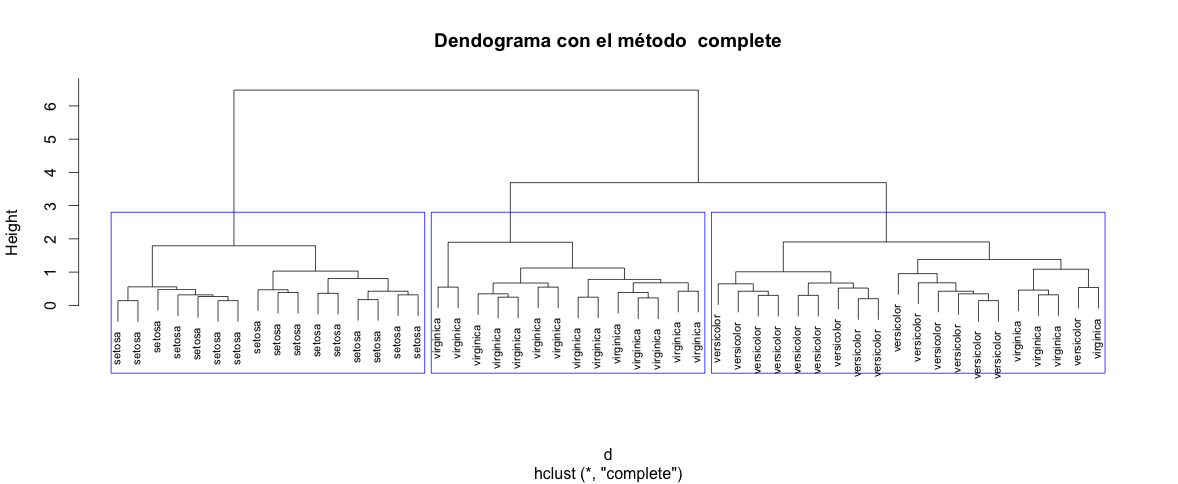
\includegraphics[width=0.45\linewidth]{imagenes/dendograma_complete}}
\subfigure[Método average]{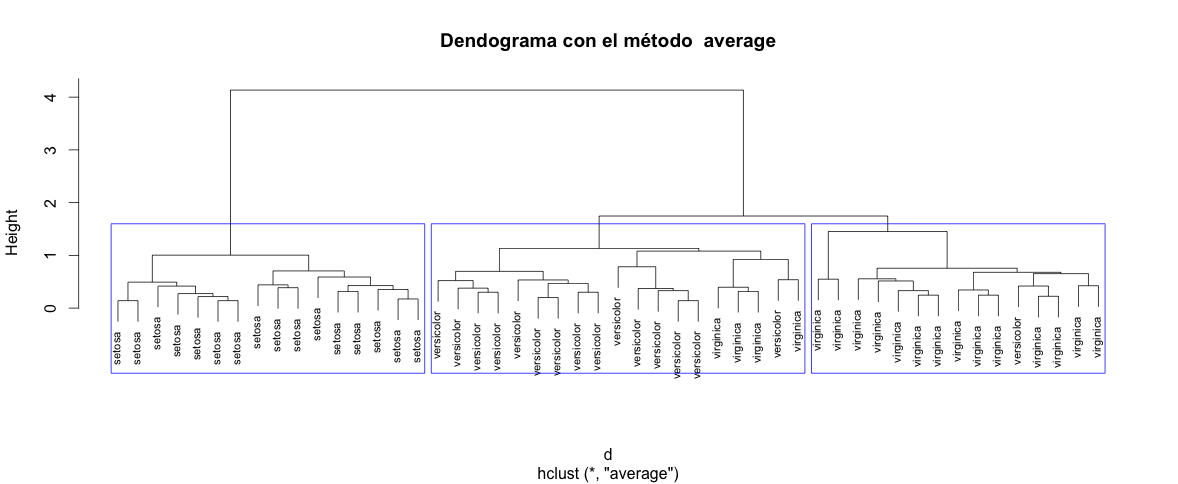
\includegraphics[width=0.45\linewidth]{imagenes/dendograma_average}}
\subfigure[Método Mcquitty]{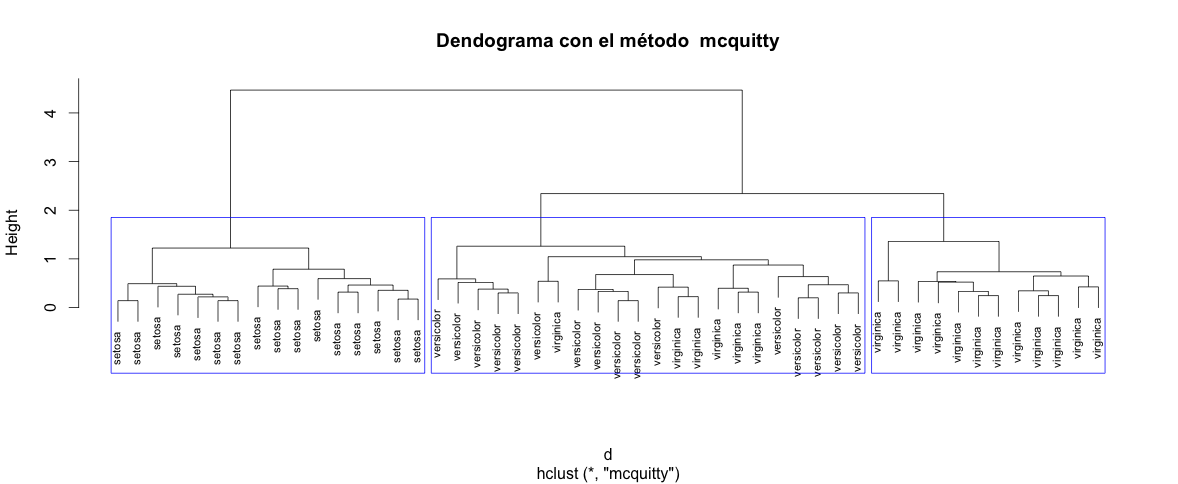
\includegraphics[width=0.45\linewidth]{imagenes/dendograma_mcquitty}}
\subfigure[Método median]{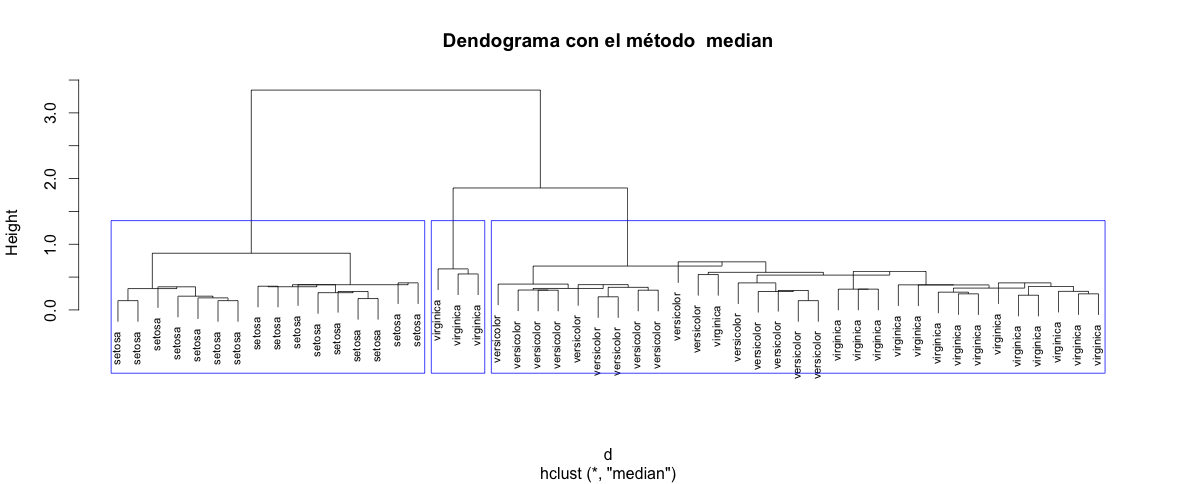
\includegraphics[width=0.45\linewidth]{imagenes/dendograma_median}}
\subfigure[Método centroid]{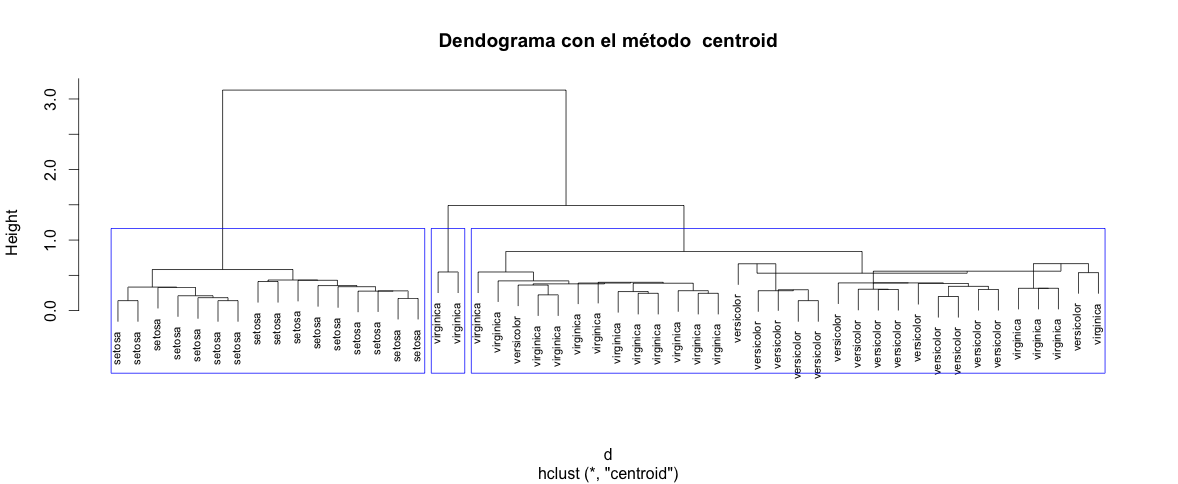
\includegraphics[width=0.45\linewidth]{imagenes/dendograma_centroid}}
\caption{Dendogramas con los métodos faltantes} \label{fig:dendogramas_otros_metodos}
\end{figure}

\section{Conclusiones}

En este caso práctico hemos visto cómo hacer un análisis de clústers. En la primera cuestión hemos identificado países en cinco grupos distintos a partir de datos socioeconómicos como el PBI, la esperanza de vida o la tasa de natalidad. En la segunda cuestión hemos visto cómo obtener dendogramas para obtener tres grupos que se debían corresponder cada uno con un tipo de iris. Dos clusters sí detectaban perfectamente el tipo de iris, pero uno de ellos mezclaba dos tipos de iris.

\clearpage

\section{Código R utilizado}

\verbatiminput{caso_5.R}

\end{document}